\chapter{Sprint 01: 10. Dez, 2015}

\textbf{Sprint beginn:} 18.11.2015
\textbf{Sprint ende:} 09.12.2015

\begin{tabular}{|l|l|l|l|l|l|}
            & Datumn        & Name            & \multicolumn{3}{l}{Unterschrift} \\ \hline
Erstellt    & 10. Dez, 2015 & Daniel Melichar & \multicolumn{3}{l}{}             \\ \hline
Geprüft     & 10. Dez, 2015 &                 & \multicolumn{3}{l}{}             \\ \hline
Freigegeben &               &                 & \multicolumn{3}{l}{}            
\end{tabular}

\subsection{Burndownchart}
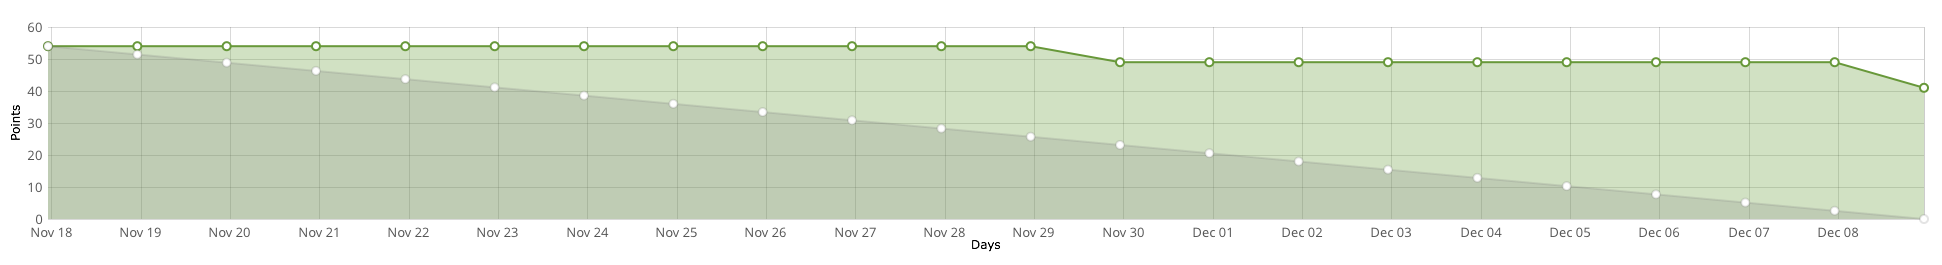
\includegraphics[scale=0.2, ]{images/sprint01-burndown.png}

\subsection{User Stories}
\resizebox{\columnwidth}{!}{%
\begin{tabular}{|l|l|l|l|l|l|}
\hline
\textbf{\#} & \textbf{User Story}                                                                                                                                                                                                                                                                                                                                                                                                                         & \textbf{Story points} & \textbf{Verantwortung} & \textbf{Akzeptanz} & \textbf{Kommentar} \\ \hline
157         & \begin{tabular}[c]{@{}l@{}}Virtual Machine\\ \\ \\ Als Entwickler möchte ich eine virtuelle Umgebung haben damit ich problemlos arbeiten kann.\\ Akzeptanzkriterien:\\ - Operating System unabhängig (Windows, OSX)\\ - Beinhaltet jede benötigte Software und Tools\\ - Software und Tools sind bereits konfiguriert\\ - Einfach zu verwenden- Versionierbar- Übertragbarkeit auf neues (actual) System geboten\end{tabular}               & 5                     & Daniel                 &                    &                    \\ \hline
15          & \begin{tabular}[c]{@{}l@{}}Datenspeicherung der Sensoren\\ \\ Als Entwickler möchte ich eine Datenbank zum handling der Sensordaten erstellen weil \\ fast jedes Features die aufbereiteten Daten benötigt.\\ Akzeptanzkriterien: \\ - Datenschema auf andere DBMS übertragbar\\ - Neue Sensoren können in die DB speichern\\ - Sensordaten wurden gefiltert\end{tabular}                                                                      & 8                     & Daniel                 &                    &                    \\ \hline
35          & \begin{tabular}[c]{@{}l@{}}Car-PC umsetzen\\ Als Entwickler möchte ich einen CarPC entwerfen und bauen der in einen DIN Slot eines \\ KFZ passt weil ich den Fahrer in der Fahrerkabine nicht in seinem Freiraum einschränken möchte\end{tabular}                                                                                                                                                                                              & 21                    & Tobi                   &                    &                    \\ \hline
6           & \begin{tabular}[c]{@{}l@{}}Sicherung der Sensordaten\\ \\ Als Admin möchte ich einen Datenbank dump erstellen können weil ich die Daten damit zu \\ einem späteren Zeitpunkt wieder einfügen kann, bzw. auf einen anderen migrieren.\\ Akzeptanzkriterien: \\ - Sicherung von spezifischen bzw. allen Daten\\ - Sensordaten verschlüsselt\\ - Sensordaten einfach auf (anderes) System migrierbar\end{tabular}                                 & 3                     & Daniel                 &                    &                    \\ \hline
18          & \begin{tabular}[c]{@{}l@{}}Weiterentwicklung der Menüs\\ \\ Als User möchte ich die erstellten Graphen der Apps leicht einsehen können weil das erlernen möglichst \\ unkompliziert gestaltet sein sollte. Eindeutig eingeordnete Felder der Unterkapitel\\ Akzeptanz: \\ - Menüstruktur Handy-App\end{tabular}                                                                                                                               & 5                     & Bozzy                  &                    &                    \\ \hline
25          & \begin{tabular}[c]{@{}l@{}}CAN Bus Manual\\ \\ Als User möchte ich ein Manual zum anstecken der CAN Bus Schnittstelle zur Verfügung gestellt \\ bekommen weil ich nicht die nötigen Kentnisse habe dies zu wissen\end{tabular}                                                                                                                                                                                                                 & 2                     & Tobi                   &                    &                    \\ \hline
27          & \begin{tabular}[c]{@{}l@{}}Car-PC Manual\\ \\ Als User möchte ich eine Anleitung zum Bedienen des Car Pc im Lieferumfang \\ enthalten haben weil ich nicht weiß wie ich den Car PC im KFZ installieren kann/soll\end{tabular}                                                                                                                                                                                                                  & 2                     & Tobi                   &                    &                    \\ \hline
2           & \begin{tabular}[c]{@{}l@{}}Menüstruktur\\ Als User möchte ich eine übersichtliche Menüstruktur weil ich mich dadurch besser zurechtfinde\\ \\ AKZEPTANZKRITERIEN\\ - Leicht benutzbare UI auch mit dickeren Fingern bei starker Vibration eines Autos\\ - Intuitive, nicht erklärungsbedürftige, Unterteilung der unterschiedlichen Funktionalitäten\\ - Ansehbares und informative UI, ausserdem gut verwendbare Schriftgröße\end{tabular} & 8                     & Bozzy                  &                    &                    \\ \hline
\end{tabular}
}